\chapter{Formulácia problému a riešenie}

\section{Formulácia problému}
\par{
Digitálne dvojča (DT) je technológia, ktorá sa čoraz častejšie využíva ako nástroj na modelovanie, navrhovanie a prototypovanie \cite{dt-iot}. V rámci 5G technológie ide o presnú digitálnu repliku siete, ktorá si s reálnou sieťou vymieňa dáta obojsmerne, v reálnom čase, v snahe zlepšiť manažment siete či zrýchliť vývoj 5G sietí \cite{systematicReview}.
}
\par{
Hoci 5G siete ponúkajú nízku latenciu a vysokú rýchlosť, sú limitované v predikcii správania, a to pre dynamiku používateľov, zaťaženie či zmeny prostredia \cite{dt-network}. DT by mohlo tieto výzvy prekonať predpoveďami budúceho stavu siete, čím by na základe aktuálneho zaťaženia siete umožnilo dynamické riadenie alokácie zdrojov a zlepšilo celkovú výkonnosť systému\cite{5g-challenges}.
\\ 
Zásadnú výzvu predstavuje práca s veľkým objemom dát, v reálnom čase, ktorá si vyžaduje vysokú výpočtovú silu, zaťažujúcu hardvér \cite{challenges-technol} a rovnako tak zachovanie nízkej latencie pri dosahovaní vysokej presnosti simulácie, potrebnej na predikciu budúceho stavu siete. Samotný model a konfigurácia DT predstavujú časovo a implementačne komplexné časti spomínaného riešenia \cite{challengesAndApplicationsReview}.
}

\section{Technický literárny prehľad}
\par{
Pojem digitálneho dvojčaťa sa v posledných rokoch, predovšetkým v technických oblastiach, spomína stále častejšie. Vzhľadom na digitalizáciu, ktorá je prítomná v každom sektore, sa transformácia hmatateľného sveta do sveta bitov a pixelov stáva prirodzeným výsledkom tohto trendu. 
}
\par{
V technickej literatúre sa DT definuje ako virtuálna reprezentácia fyzického objektu, medzi ktorými prebieha automatizovaný bilaterálny tok dát v reálnom čase \cite{DT:OriginToFuture}. Tok dát zabezpečuje presné zrkadlenie správania oboch týchto entít \cite{systematicReview}. Vlastnosť zrkadlenia, viď Obr. \ref{fig:PLM}, poskytuje mnohé výhody ako napríklad možnosti monitorovania v reálnom čase, preventívnej údržby \cite{5g&beyond}, či urýchlenie procesu vývoja, pretože eliminuje potrebu prototypovania v každej fáze vývoja \cite{mitigating_book}.
}
\newline
\begin{figure}[H]
    \centering
    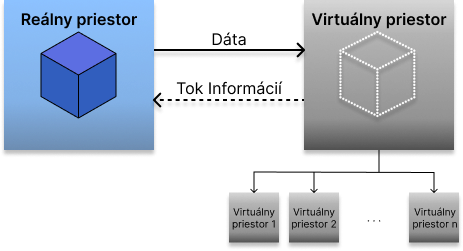
\includegraphics[width=0.8\linewidth]{assets/images/Grieves_PLM_model.png}
    \caption[Model zrkadlených priestorov]{Model zrkadlených priestorov (Mirrored Spaces Model) tak, ako ho vo svojej práci navrhol Grieves \cite{Grieves}. Tento model sa skladá z troch komponentov - reálny priestor (Real Space), virtuálny priestor (Virtual space) a spájací mechanizmus (Linking Mechanism) \cite{DT:OriginToFuture}, ktorý prúdi automatizovane oboma smermi medzi týmito priestormi. Virtuálny priestor vytvára digitálnu reprezentáciu reálnych objektov a podporuje viacero virtuálnych systémov na analýzu, simuláciu alebo predikciu správania fyzických objektov.}
    \label{fig:PLM}
\end{figure}

\par{Vo  svojom výskume Enders a Hoßbachová \cite{DimensionOfDTAplication} identifikovali sektory, kde je používanie digitálneho dvojčaťa najrozšírenejšie. Patria sem výroba \cite{manuf}, letecký priemysel \cite{aircraft}, energetika \cite{energy}, automobilový priemysel \cite{automotive}, námorníctvo \cite{marine}, petrochemický priemysel \cite{oil}, poľnohospodárstvo \cite{agriculture}, zdravotníctvo \cite{health}, verejný sektor \cite{education} a ťažba \cite{mining}.
}
\par{Taktiež identifikovali tri hlavné využitia digitálneho dvojčaťa v týchto oblastiach \cite{AplicationsOfDT}: ovládanie, simulovanie a monitorovanie. To však ani zďaleka nepokrýva všetky možnosti a spôsoby využitia. Digitálne dvojča dnes nájde uplatnenie aj pri dizajnovaní, validácii, predchádzaní chýb, trénovaní, optimalizácii a predikcii.
}
\par{Ak sa chceme pozrieť na reálne aplikácie DT, Huawei implementoval DT na monitorovanie výrobných liniek \cite{huawei2020}, zatiaľ čo mestá ako Bristol \cite{Bristol} či Singapur \cite{singapur} používajú DT na efektívne riadenie inteligentných mestských systémov. V týchto scenároch DT umožňuje predikciu zlyhaní, optimalizáciu zdrojov a minimalizáciu prestojov. Podobné prístupy sú použiteľné aj v telekomunikáciách, kde DT dokáže simulovať a predikovať správanie sietí v reálnom čase. 
}
\par{V oblasti telekomunikácií sa čoraz viac využívajú pri simuláciách rádiových prístupových sietí (RAN), monitorovaní jadra siete a optimalizácii zdrojov. Napríklad Siemens nasadzuje DT na správu a optimalizáciu sieťových komponentov \cite{5g&beyond}. Podobne, ZTE a China Mobile \cite{ChinaMobile} úspešne aplikovali technológiu digitálneho dvojčaťa na zlepšenie 5G konektivity pre vysokorýchlostnú železničnú trať v južnej Číne. Pomocou presného 3D modelu infraštruktúry popri trati optimalizovali výkonnosť 5G siete, čím dosiahli pokrytie na úrovni 98,5\% a rýchlosti sťahovania presahujúce 300 Mbps. 
}
\par{ Tieto úspešné implementácie demonštrujú širokú škálu výhod technológie DT v telekomunikáciách, od optimalizácie pokrytia po zvyšovanie kvality služieb. Napriek tomu však existujú určité obmedzenia, ako napríklad zložitosť nasadenia \cite{impl}, škálovateľnosť \cite{econ} a presnosť simulácií \cite{predictions_risks}, ktoré je potrebné prekonať pri vývoji nových riešení. 
}

\section{Prehľad riešenia (na vysokej úrovni)}
% Poznámka čo znamená high level = denoting a programming language that is relatively accessible to the user, having instructions that resemble a natural language such as English.

% Stručne vysvetlite riešenie problému. Študenti by mali byť schopní odôvodniť svoj výber techník použitých na riešenie problému, uznať ich obmedzenia a interdisciplinárny dosah. | 2-3 strany
\par{
Cieľom tohto projektu je vytvoriť DT 5G siete, ktoré bude schopné v reálnom čase napodobňovať správanie skutočnej siete na základe historických a aktuálnych pozorovaní a predikcií jej budúcich stavov. Tento systém poskytne hodnotné nástroje pre optimalizáciu a analýzu výkonu 5G sietí, pričom jeho implementácia zahŕňa kombináciu otvorených softvérových riešení a pokročilých metód spracovania dát v spojení s vytvorením vhodného modelu strojového učenia.
}

\par{
DT bude simulovať kľúčové aspekty 5G siete prostredníctvom troch hlavných komponentov: Open5GS pre implementáciu jadra siete, srsRAN pre simuláciu rádiového prístupu (RAN) a UERANSIM pre emuláciu užívateľských zariadení (UE) a testovanie rôznych scenárov. Kombináciou týchto nástrojov bude možné modelovať tok dát v sieti a analyzovať metriky ako latencia, priepustnosť a stabilita spojenia. Tieto údaje budú slúžiť ako vstup pre strojové učenie, ktoré umožní predpovedať budúce stavy a zmeny v sieti.
}

\par{
Každý komponent DT plní špecifickú úlohu. Open5GS zaisťuje základné funkcie na správu riadiacej roviny (control plane) a užívateľských dát (user plane). Jeho flexibilná architektúra umožňuje jednoduché prepojenie s inými nástrojmi a podporuje najnovšie štandardy 5G. srsRAN simuláciou pokrýva rádiový prístup a umožňuje testovať rôzne konfigurácie siete, čo pomáha zistiť ich vplyv na celkovú výkonnosť. Na druhej strane, UERANSIM sa zameriava na emuláciu správania zariadení pripojených k sieti. Generuje realistickú prevádzku, či už ide o videohovory alebo masívne pripojenie IoT zariadení. Táto kombinácia nástrojov umožňuje komplexnú analýzu a testovanie, čo je kľúčové pre vytvorenie spoľahlivého predikčného modelu. Architektúra a konkrétne prepojenia častí jednotlivých komponentov je zobrazené v Obr. \ref{fig:architecture} nižšie.
}
\newline
\begin{figure}[H]
    \centering
    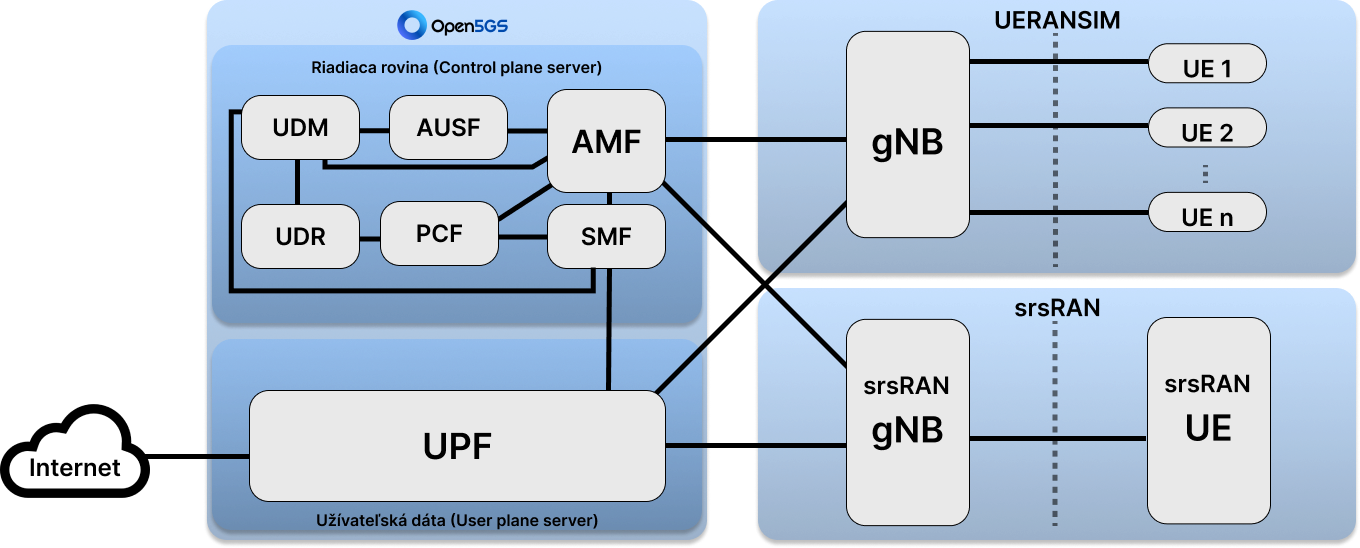
\includegraphics[width=0.75\linewidth]{assets/images/open5gs+ueran.png}
    \caption[Architektúra komponentov Open5GS, srsRAN a UERANSIM]{Architektúra jednotlivých komponentov Open5GS \cite{open5gs}, srsRAN a UERANSIM a ich vzájomné prepojenie. Open5GS je rozdelené na riadiacu rovinu a rovinu užívateľských dát a obe tieto roviny sú napojené na gNB (5G bunky), ku ktorým sa môžu pripájať zariadenia. Architektúra zobrazuje možnosť použiť UERANSIM na priame pripojenie ku Open5GS jadru a alternatívne RAN pripojenie pomocou srsRAN.}
    \label{fig:architecture}
\end{figure}

\par{
Architektúra DT je navrhnutá tak, aby jednotlivé komponenty medzi sebou hladko spolupracovali. Rádiová prístupová sieť, ktorá je simulovaná pomocou srsRAN, zhromažďuje a odosiela dáta do jadra siete, ktoré je realizované cez Open5GS. Toto jadro tieto dáta spracuje a posiela ďalším komponentom. UERANSIM generuje realistické komunikačné scenáre medzi zariadeniami a simulovanou sieťou. Napríklad môžeme testovať situácie, kde je sieť preťažená alebo dočasne vypadne spojenie. Zozbierané dáta sa potom použijú na tréning predikčného modelu, ktorý následne analyzuje tieto scenáre a pomáha doladiť parametre, aby model lepšie reagoval na budúce situácie.
}

\par{
Pre spracovanie dát sa využijú nástroje MATLAB a Simulink, ktoré poskytujú intuitívne prostredie na tvorbu modelov pomocou strojového učenia. Proces začína získavaním dát zo simulácií, ktoré prejdú krokom čistenia na odstránenie chybných alebo neúplných hodnôt. Následne sa tieto dáta normalizujú, čo znamená, že ich hodnoty budú upravené tak, aby boli vhodné na analýzu a modelovanie. Model bude navrhnutý tak, aby dokázal predpovedať dôležité parametre siete, ako napríklad latenciu či priepustnosť, a to na niekoľko sekúnd dopredu. Takáto predikcia môže prispieť k optimalizácii prevádzky siete, zlepšeniu kvality služieb a k úspore energie. Navrhovaná architektúra je zobrazená na Obr. \ref{fig:solution}. \\
}


\begin{figure}[H]
    \centering
    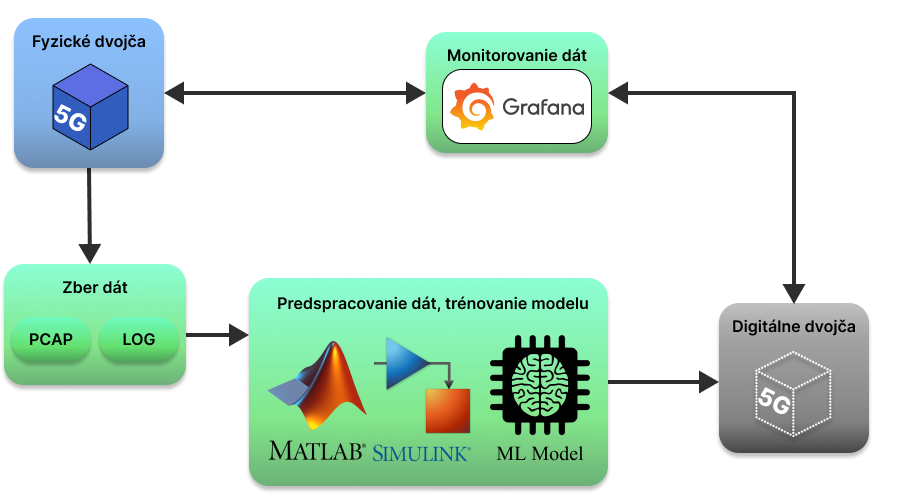
\includegraphics[width=0.85\linewidth]{assets/images/high-level-model.png}
    \caption[Návrh riešenia (High level)]{V návrhu riešenie je zobrazený tok dát medzi jednotlivými časťami projektu. Na jednej strane je Fyzické dvojča, na druhej Digitálne dvojča a v strede sú jednotlivé nástroje, ktoré slúžia na monitorovanie aktuálneho stavu a predikciu budúceho stavu. Na zber dát slúžia súbory typu PCAP zachytené softvérom (napr. Wireshark \cite{wireshark}) a LOG, ktoré sú zaznamenané v logoch z jednotlivých častí 5G siete. Tieto dáta sú predspracované a použité na trénovanie modelu ML a následné predikcie budúcich stavov. Na základe týchto predikcií sa upravia parametre a nastavenia oboch fyzickej a digitálnej siete. Nástroj Grafana \cite{grafana} poskytuje rozhranie pre monitorovanie a vizualizáciu dát a aktuálneho stavu siete.}
    \label{fig:solution}
\end{figure}

\par{
Riešenie však čelí viacerým výzvam. Presnosť predikcií je ovplyvnená kvalitou a objemom dát, ktoré sú dostupné. Simulácie môžu byť výpočtovo náročné a obmedzené výkonom hardvéru. Navyše, implementácia a testovanie predikčného modelu si vyžaduje značný čas. Obmedzenia softvérových nástrojov, ako sú MATLAB a Simulink, môžu taktiež ovplyvniť rozsah a možnosti simulácie. Tieto faktory budú starostlivo zohľadnené a brané do úvahy počas celého životného cyklu tohoto projektu, od jeho implementácie až po nasadenie.
}

\section{Hodnotenie rizík}
\par{
Implementácia digitálneho dvojčaťa 5G siete spolu s modelom ML prináša rôzne výzvy, ktoré môžu ovplyvniť presnosť predpovedí, stabilitu a efektívnosť celého systému. Identifikácia týchto problémov a návrh stratégií na ich zmiernenie sú jednou z kľúčových úloh tejto práce.

Nedostatočná kvalita vstupných dát je jedným z najpravdepodobnejších rizík, ktoré môžu viesť k nesprávnym výsledkom modelu. Chyby v dátach alebo ich nereprezentatívnosť, napríklad pri modeloch sieťovej prevádzky (traffic patterns), môžu narušiť presnosť predpovedí \cite{ML_traffic}. Formou zmiernenia je testovanie na rôznych dátových scenároch a aplikácia metód ako krížová validácia a ladenie hyperparametrov, ktoré minimalizujú riziko chýb spojených s podtrénovaním (underfitting) a pretrénovaním (overfitting) \cite{Nguyen}.

Zber kvalitných dát môže byť problematický, pretože mnohé scenáre je potrebné zachytiť v laboratóriu. Bez dostatočných dát môže model generovať neadekvátne predpovede, ktoré nebudé reprezentovať skutočnosť. Riešením môže byť generovanie syntetických údajov \cite{data_generating} a využitie dostupných datasetov z iných projektov \cite{datasets_telecom}, ktoré môžu čiastočne nahradiť reálne dáta a napomôcť k presnejším predpovediam.

Nezvyčajné scenáre, ako vysoké zaťaženie siete (peak loads), neštandardné správanie používateľov či poveternostné podmienky môžu narušiť schopnosť modelu adaptovať sa \cite{challenges_human_factor}. Ak tieto scenáre neobsahujú trénovacie dáta, model nemusí byť pripravený na takéto situácie. Vzhľadom na čas, ktorý máme na získanie a predspracovanie dát, tento problém nemusí byť vo finálnej implementácií vyriešený dostatočne, a preto jeho vyriešenie vyžaduje ďalšiu prácu a zber dát.

Kompatibilita systémov ako srsRAN, Open5GS, UERANSIM a nástrojov Docker nie je vždy automatizovaná, čo môže ovplyvniť celkovú integráciu práce \cite{challenges_human_factor}. Z tohoto dôvodu je vhodné začínať implementáciu na malých izolovaných komponentoch, za neustáleho testovania. Takéto testovanie, a celkový vývoj DT sú časovo veľmi náročné, čo potvrdili aj autori v \cite{USAirForce}. Tento fakt môže negatívne vplývať na výsledok celej práce, nakoľko čas je jedným z kľúčových faktorov, ktoré majú vplyv na množstvo a kvalitu pozberaných dát určených na trénovanie ML modelu.

Konfigurácia siete môže odhaliť citlivé informácie o 5G infraštruktúre či porušenie GDPR \cite{big-data-problems} pri nechcenom zachytení údajov o používateľoch \cite{challenges-technol}. Únik takýchto dát by ohrozil nielen bezpečnosť projektu, ale aj reálnej siete \cite{Dt_Iot_data_worry_about}. Používanie .env súborov na uchovávanie citlivých premenných a simulovanie siete s fiktívnymi údajmi výrazne znižuje riziko úniku.
}

%\par{Študenti by mali rozpoznať riziká spojené s implementáciou ich riešení a ponúknuť stratégie na ich zmiernenie. | max. 1 strana}

\begin{comment}
\section{Experimentálna reprodukovateľnosť a integrácia}
\par{
Fáza inžinierstva riešení by mala byť vykonávaná s ohľadom na reprodukovateľnosť a systémovú integráciu a študenti by mali podrobne opísať, ako sa tejto otázke venovali. Pokiaľ nie sú špeciálne podmienky, kód, modely a dáta použité pri inžinierstve riešení by mali byť voľne dostupné. Modely strojového učenia by mali byť prezentované tak, aby umožňovali ďalšie využitie bez nutnosti rekvalifikácie. Tam, kde je to možné, použite riešenia v kontajneroch, ktoré zabezpečia použiteľnosť produktu alebo služby aj pri zmene základnej technológie. | 3 strany
}
\par{
Setup Documentation: \\
- step-by-step instalacia na jednotlivých VMs
- neviem či sa bude dať docker (?) - ale pravdepodobne aspoň na niečo by sa dalo - setupy VMs a resp, celé VM dať do dockeru

Source Code - dostupnosť: \\
GitHub - Readme, version control

Úvahy o integrácií: \\
- Modularita komponentov - každý z nich má svoju funkciu a umožňuje rozširovanie
Logovanie a Interface konzistencia: \\
- popisať ako logujeme data, aby to bolo reprodukovateľné

Future-Proofing: \\
- izolovanie komponentov, mozne zmeny bez nutnosti meniť celý projekt

Machine Learning a znovu použiteľnosť:\\ 
- Popísať ako je model trenovaný, aká je jeho architektúra, parametre a hyperparametre + trénovacie dáta
- zabezpečiť, aby bol už model natrénovaný, aby ho ostatní v budúcnosti nemuseli trénovať znova.
- spomenúť knižnice, štandardy
}
\end{comment}

\section{Udržateľnosť a environmentálny dopad}
%Študenti by mali opísať, ako by implementovali opatrenia na zabezpečenie udržateľnosti svojho produktu alebo služby počas životného cyklu. | 1-2 strany
\par{
Implementácia opatrení na zabezpečenie udržateľnosti projektu a minimalizácia jeho environmentálneho dopadu sú kľúčové pre zaistenie dlhodobej hodnoty, spoločenského prínosu a efektivity vypracovania tejto práce. Práca je navrhnutá s dôrazom na efektívne využívanie zdrojov, udržateľný softvérový a hardvérový návrh a životný cyklus 5G siete, ktorý minimalizuje potrebu používania fyzických zdrojov.
}

\par{
Jednou z hlavných prínosov DT je možnosť predikcie a optimalizácie, pričom ak je DT zostrojené správne, môže dopomôcť k redukcií spotreby elektrickej energie. \cite{DT_edge_networks_IoT}. Predikcia budúceho stavu siete umožňuje taktiež lepšiu správu záťaže (traffic load) a preťaženia (congestion), čo napomáha k znižovaniu nadmernej spotreby energie \cite{malaysia_enviro}. Navyše, DT eliminuje potrebu testovania na fyzických zariadeniach, čím sa minimalizuje spotreba rôznych materiálov \cite{enviro_raw_materials} a času potrebného na fyzické experimenty. Tento prístup je obzvlášť užitočný v prípade nasadzovania a testovania 5G technológií v oblastiach s nerozvinutou infraštruktúrou a obmedzenými výrobnými zdrojmi \cite{huaweii_i_cities}.
}

\par{
Vývoj softvéru bol orientovaný na maximálnu efektivitu, čo zahŕňa optimalizáciu kódu na zníženie spotreby energie počas behu aplikácie a nasadenie projektu v prostredí Docker, čo umožňuje rýchlejšiu konfiguráciu a škálovateľnosť zariadení. Tieto opatrenia nielen znižujú environmentálny dopad \cite{docker_enviro}\cite{docker_enviro_2}, ale aj zvyšujú celkovú udržateľnosť projektu.
}

\par{
Modulárny dizajn \cite{modular_sw} projektu zabezpečuje, že aktualizácie a údržba nemajú vplyv na celkovú funkčnosť systému. Tento prístup znižuje potrebu kompletného prekonfigurovania alebo fyzických zásahov do chodu programu, čo prispieva k dlhodobej udržateľnosti. Takýto dizajn môže mať pozitívny vplyv na životné prostredie \cite{modular_sw} (Green Design).
}

\par{
Ako je vyššie uvedené, použitie prediktívnych modelov v DT môže viesť k zásadným environmentálnym prínosom \cite{enviro}. Okrem zníženia zaťaženie fyzickej infraštruktúry a menej častých aktualizácie fyzického hardvéru, môže mať za následok aj nižšiu spotrebu zdrojov a menšiu produkciu odpadu \cite{enviro_raw_materials}. Predikčné modely teda umožňujú efektívnejšie rozhodovanie s pozitívnym dopadom na životné prostredie.
}

\section{Zamestnateľnosť}
\par{
Táto bakalárska práca, zameraná na rozvoj teoretických znalostí v oblasti digitálnych dvojčiat v spojení s praktickou implementáciou a optimalizáciou 5G sietí, vedie k rozšíreniu zručností vo viacerých kľúčových oblastiach technologického sektora. V neposlednom rade strojové učenie, použité na predikciu správania implementovaného digitálneho dvojčaťa, zasahuje aj do oblasti dátovej vedy.

Vďaka formátu práce autori prejdú celým cyklom realizácie projektu, od prieskumu technológií cez návrh až po implementáciu a testovanie. Týmto získajú ucelený a komplexný pohľad na vývoj a riadenie softvérových projektov, ako aj na plánovanie, organizáciu a efektívnu komunikáciu.

Takáto kombinácia technických, projektových a komunikačných schopností môže významne zvýšiť hodnotu autorov na trhu práce, najmä v budúcnosti, keďže problematika digitálnych dvojčiat a 5G sietí je stále viac žiadaná a nachádza uplatnenie v rôznych odvetviach.
}\begin{comment}
\section{Tímová práca, diverzita a inklúzia}
\par{
Ak sa na projekte podieľajú odborníci z viacerých odborov, študent by mal implementovať procesy a opísať techniky pre zdieľanie úloh a (pochopenie) znalostí medzi rôznymi stranami. Mali by sa opísať problémy a stratégie na ich zmiernenie, aby sa zabezpečilo dokončenie projektu v stanovenom časovom harmonograme. Táto časť by mala obsahovať aj úvahy o diverzite a inklúzii. | ½-1 strana
}
\par{
Teamwork and Knowledge Sharing: \\
- spolupráca s Matejom a Matejom

Diversity and Inclusion:
- Ageism - pomoc pre všetky vekové skupiny?
- Disabled people? hearing, vision ...
- môže im to DT nejko pomôcť?
- Prehľadná dokumentáia a návod pre možnú spoloprácu...
}

Spolupráca s konzultantom a inými odborníkmi: Môžete zdôrazniť, ako ste spolupracovali s konzultantom, odborníkmi alebo kolegami, aby ste získali spätnú väzbu alebo konzultovali technické aspekty projektu.

Diverzia myšlienok a prístupov: Aj keď ste projekt riešili individuálne, môžete opísať, ako ste zohľadnili rôzne perspektívy pri výbere riešení a metodík. Napríklad môžete zdôrazniť, že ste čerpali z rôznych zdrojov, ako sú články, výskumy a prípadové štúdie, aby ste vytvorili univerzálne použiteľný a inkluzívny návrh.

Prístupnosť a inklúzia výsledkov projektu: Opíšte, ako váš projekt môže byť prínosný pre širšiu komunitu používateľov. Napríklad, ak je váš digitálny dvojča schopné zlepšiť efektivitu nasadzovania 5G sietí, môže byť relevantný aj pre menej rozvinuté regióny alebo oblasti so zníženými zdrojmi.

Schopnosť prispôsobiť projekt tímovému pracovnému prostrediu: Môžete uviesť, že ste navrhli systém s ohľadom na modularitu a jednoduchú integráciu, čo umožňuje budúcu spoluprácu tímov na rozšírení projektu

Článok - Intro a Related work
\end{comment}